New challenges arise when performing DWT on distributed memory systems,
since job decomposition and inter-processor communication are both controled
by the program.
%
Load balance and communication costs then become the biggest concerns 
regarding DWT on distributed memory systems.

Chadha et. al. analyzed two straightforward strategies of decomposing 
the DWT on two-dimensional data array: stripe decomposition and
checkerboard decomposition~\cite{chadha2002scalable}.
%
These two decomposition strategies require different ways to communicate
with neighbor processors.
%
On the one hand, stripe decomposition requires communicating to two 
neighbor processors, while checkerboard decomposition requires four.
%
On the other hand, stripe decomposition requires communicating larger
amount of data, compared to checkerboard decomposition.
%
Chadha et. al. showed that the stripe decomposition provides better
performance than the checkerboard partitioning.
%
More specifically, the theoretical speedup for stripe decomposition 
is nearly linear with larger number of processors.

Nielsen et. al. independently revealed linear speedup when performing 
two-dimensional DWT, using the stripe decomposition~\cite{nielsen1997scalable}.
%
Moreover, this research analyzed two approaches of data communication in
two-dimensional DWT.
%
The first approach performs a matrix transpose in between of DWTs on
two the dimensions. 
%
This approach keeps good data locality for each single calculation, but 
results in large amount of data transferring when switching the calculation
to the other dimension.
%
The second approach keeps data local on each processor, and exchange values
with its neighbor processors.
%
This approach has minimal amount data to transfer, but the data transfer happens 
more frequently.
%
Figure~\ref{fig:c} illustrates these two approaches. 
%
Analysis showed the second approach, which saves a massive transpose operation,
performs better with larger number of processors.

\begin{figure}
    \centering
    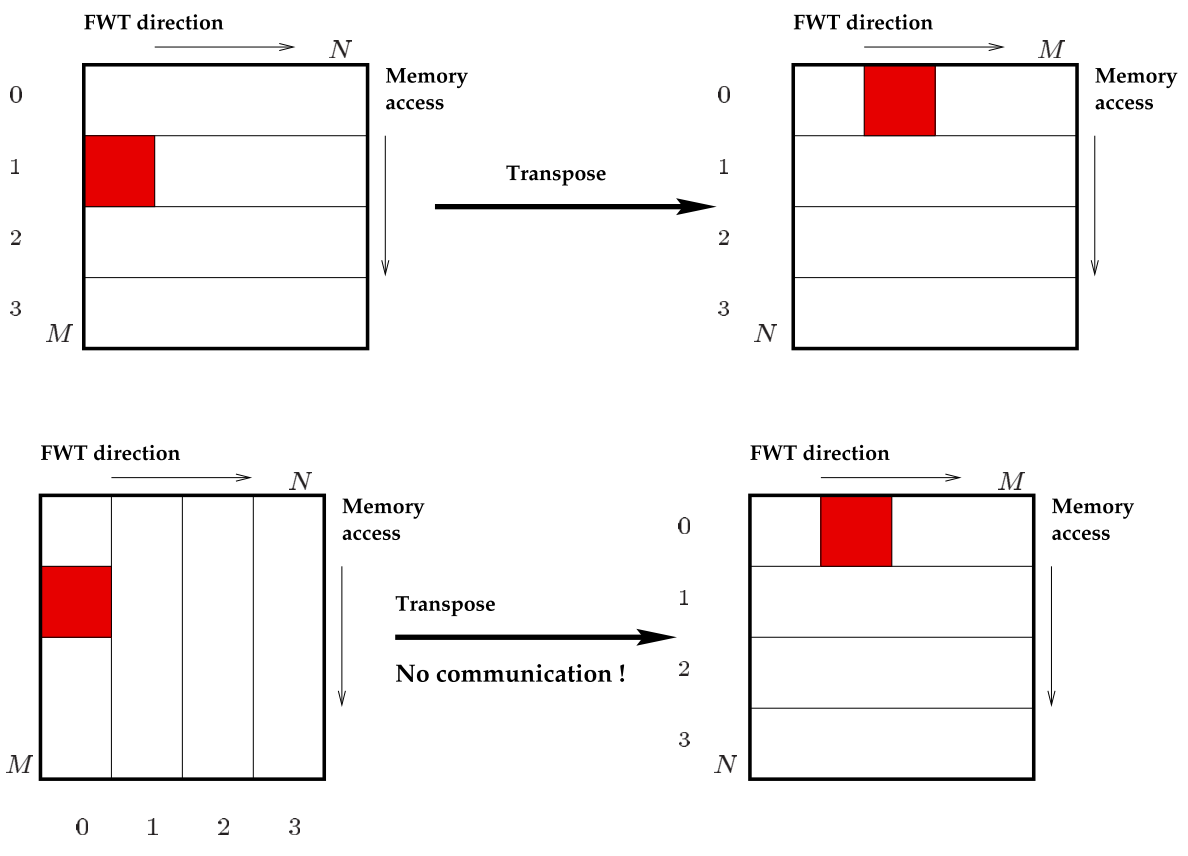
\includegraphics[width=0.95\textwidth]{fig/c.png}
    \caption{Two approaches of data communication: 
             the top approach involves a transpose for the entire data,
             while the bottom approach involves boundary communication between neighbor processors.}
    \label{fig:c}
\end{figure}



